\subsection{Closing channels}
\label{sec:syncchan-closing}

\inlineScala

We now consider the closing of SCL channels.  Recall that, after the channel
has been closed, a |send| or |receive| execution fails and throws a |Closed|
exception.

Implementing the |close| operation correctly proved harder than expected.  An
earlier version of the implementation suffered from a bug involving three
threads acting concurrently: thread~$A$ calls |send(x)|, thread~$B$ calls
|receive|, and thread~$C$ calls |close|.  Under certain conditions, it was
possible for thread~$B$ to return successfully, having received~|x|, but for
thread~$A$ to see the channel closed, and so throw a |Closed| exception.  We
consider this behaviour to be incorrect: either both~$A$ and~$B$ should think
the communication has succeeded, or both should throw |Closed| exceptions.

%%%%%%%%%% Implementation

The SCL implementation uses a boolean variable |isChanClosed| that records
whether the channel is closed.  The |close| operation sets this variable, and
signals to all the threads waiting on conditions.
\begin{scala}
def close = lock.mutex{
  if(!isChanClosed){isChanClosed = true; slotEmptied.signalAll(); slotFull.signalAll(); continue.signalAll()}
}
\end{scala}

The implementation also uses a variable |receiversWaiting|, which records how
many receivers are currently waiting to receive a value. 

Figure~\ref{fig:close-send-receive} gives code to show how |send| and
|receive| deal with the channel being closed.  (Note: this is still a large
simplification of the full code, which supports alts and the timed
operations.)

%%%%%

\begin{figure}
\begin{minipage}[t]{80mm}
\begin{scala}
def send(x: A) = lock.mutex{
  while(status != Empty && !isChanClosed)
    slotEmptied.await()  
  if(isChanClosed) throw new Closed
  value = x; status = Filled
  if(receiversWaiting > 0) slotFull.signal()
  continue.await()  
  if(status == Read){ 
    status = Empty; slotEmptied.signal() }
  else{ 
    assert(isChanClosed)
    if(receiversWaiting == 0) throw new Closed }
}
\end{scala}
\end{minipage}
%
\begin{minipage}[t]{75mm}
\begin{scala}
def receive(): A = lock.mutex{
  if(isChanClosed) throw new Closed
  while(status != Filled){
    receiversWaiting += 1; slotFull.await()
    receiversWaiting -= 1
    if(status != Filled && isChanClosed)
      throw new Closed
  }
  status = Read; continue.signal(); value
}
\end{scala}
\end{minipage}
\caption{Code for deadling with closed channels when sending and receiving.}
\label{fig:close-send-receive}
\end{figure}

%%%%%

When a thread calls |send| or |receive|, if |isChanClosed| is set, it throws a
|Closed| exception.  Likewise, if a sending thread waits on |slotEmptied|, it
performs a similar check when it receives a signal.  

If a receiving thread waits on |slotFull|, when it receives a signal, it first
checks whether |status| holds |Filled|.  If so, it continues as described
earlier: thus we prioritise completing the communication over checking whether
the channel has been closed (this seems necessary for correct interaction with
alts).
%
%% More precisely, an alt might have filled the slot, which implies it has
%% performed the computation to calculate the value: at this point, it is
%% committed to the communication. 
If |status| does not hold |Filled|, the thread checks whether the channel has
been closed, and if so throws an exception; otherwise, it waits again on
|slotFull|.

If a sending thread waits on |continue|, when it receives a signal, it first
checks whether |status| holds |Read|, and if so continues as described
earlier.  Otherwise, it must be the case that |isChanClosed| has been set (the
SCL implementation asserts this, and the CSP analysis below checks this).
However, if there is a receiver waiting (as recorded by |receiversWaiting|),
then that receiver will eventually return the value being sent, so the sending
thread should also return successfully.  If there is no waiting receiver, the
sending thread throws a |Closed| exception.
%
%% \begin{scala}
%%   continue.await()  
%%   if(status == Read){ status = Empty; slotEmptied.signal() }
%%   else{ assert(isChanClosed); if(receiversWaiting == 0) throw new Closed }
%% \end{scala}

The precise order of checks in the previous paragraphs is rather subtle.  This
is where the earlier implementation went wrong.  Previously, when the waiting
thread received a signal, it \emph{first} checked |isChanClosed|, and if it
was set, threw a |Closed| exception.  This could be wrong for a couple of
reasons, as illustrated in Figure~\ref{fig:old-impl-error}.
%
\begin{itemize}
\item
In the top part of the figure, a receiving thread reads and returns the
sending thread's value, indicating that it has correctly synchronised.  Then
the channel is closed.  If the |send| first checks |isChanClosed|, it will
throw a |Closed| exception.  This is an error: either both threads should
succeed, or both should see the channel had closed, and fail.  The correct
version (Figure~\ref{fig:close-send-receive}) instead reads |status| first,
and returns correctly.

\item
The bottom part of the figure is similar, but the channel is closed and the
|send| continues \emph{before} the |receive| reads the sender's value.  If the
|send| first checks |isChanClosed| (and maybe |status|), it will throw a
|Closed| exception, even though the |receive| will subsequently return the
sender's value.  This is again an error.  The correct version instead finds
$\sm{receiversWaiting} > 0$, and so returns correctly.
\end{itemize}
This correct version was found with the help of the model checking described
below.


%%%%%%%%%%

\begin{figure}
\def\height{10.5}
\def\width{6}
%%%%%
\begin{tikzpicture}[yscale = 0.5, xscale = 0.9, >= angle 60]
\draw (0,0) node[draw](send){\scalashape send};
\draw (send) -- ++ (0,-\height);
\draw (\width,0) node[draw](receive){\scalashape receive};
\draw (receive) -- ++ (0,-\height);
\draw (12,0) node[draw](close){\scalashape close};
\draw (close) -- ++ (0,-\height);
%
%\draw (receive) ++(0,-1) node[right]{\ldots; \scalashape slotFull.await()};
%
\draw (send)++(0,-1) node[right]{\ldots};
\draw (send)++(0,-2) node[right]{
  set {\scalashape value = x}, {\scalashape status = Filled}};
%\draw[->] (0,-3.7) -- node[above]{\scalashape slotFull.signal()}  (\width,-3.7);
\draw (send)++(0,-3) node[right]{\ldots; \scalashape continue.await()};
%
\draw (receive) ++ (0,-4) node[right]{
  \ldots; read {\scalashape status = Filled}};
\draw (receive) ++ (0,-5) node[right]{set {\scalashape status = Read};
  \ldots};
\draw (receive) ++ (0,-6) node[right]{ \scalashape continue.signal()};
\draw[->] (receive)++(0,-6) --  (0,-6);
\draw (receive) ++ (0,-7) node[right]{return {\scalashape value}};
%
\draw (close)++(0,-8) node[right]{set {\scalashape isChanClosed = true}; \ldots};
%
\draw (send) ++ (0,-9) node[right]{read {\scalashape isChanClosed = true}};
\draw (send) ++ (0,-10) node[right]{throw {\scalashape Closed} exception};
\end{tikzpicture}

\bigskip

%%%%%

\def\height{11.5}
\begin{tikzpicture}[yscale = 0.5, xscale = 0.9, >= angle 60]
\draw (0,0) node[draw](send){\scalashape send};
\draw (send) -- ++ (0,-\height);
\draw (\width,0) node[draw](receive){\scalashape receive};
\draw (receive) -- ++ (0,-\height);
\draw (12,0) node[draw](close){\scalashape close};
\draw (close) -- ++ (0,-\height);
%
\draw (receive) ++(0,-1) node[right]{\ldots; \scalashape slotFull.await()};
%
\draw (send)++(0,-2) node[right]{\ldots};
\draw (send)++(0,-3) node[right]{
  set {\scalashape value = x}, {\scalashape status = Filled}};
\draw (send)++(0,-4) node[right] (sig1) {\scalashape slotFull.signal()};
\draw[->] (sig1) --  (\width,-4);
\draw (send)++(0,-5) node[right]{\ldots; \scalashape continue.await()};
%
\draw (close)++(0,-6) node[right]{set {\scalashape isChanClosed = true};
  \ldots};
%% \draw(close)++(0,-7) node[right]{\scalashape slotFull.signalAll()};
%% \draw[->] (close)++(0,-7) -- (\width,-7);
\draw(close)++(0,-7) node[right]{\scalashape continue.signalAll()};
\draw[->] (close)++(0,-7) -- (0,-7);
%
\draw (send) ++ (0,-8) node[right]{read {\scalashape isChanClosed = true}};
\draw (send) ++ (0,-9) node[right]{throw {\scalashape Closed} exception};
%
\draw (receive) ++ (0,-10) node[right]{
  \ldots; read {\scalashape status = Filled}; \ldots};
\draw (receive) ++ (0,-11) node[right]{return {\scalashape value}};
%

\end{tikzpicture}

\caption{Illustration of errors that arise in the earlier implementation.
  Several steps are elided, for brevity.}
\label{fig:old-impl-error}
\end{figure}

%%%%%%%%%% Model

\inlineCSP

Adapting the CSP model to model closing of channels is straightforward.  The
|endSend| and |endReceive| channels are extended to allow a result |Closed|,
corresponding to the \SCALA{Closed} exception.  The \SCALA{close} operation is
modelled as for earlier operations, framed by events on channels |beginClose|
and |endClosed|.

%%%%%%%%%% Testing

To analyse this extended model, we adapt the |System| process from earlier to
also allow threads to close channels.  

The channel specification in Section~\ref{sec:syncchan-analysis-1} is (in the
terminology of~\cite{LL:synchronisation}) \emph{stateless}: no state is
carried forward from one synchronisation to another.  However, when we
consider closing of the channel, it becomes \emph{stateful}, with two states,
open or closed.  (Other synchronisation objects have more interesting states.)
The definition of synchronisation linearisation requires the synchronisation
history to be consistent with the state. 

Our specification will treat \SCALA{close} as a linearisable operation: it
will appear to take place atomically, at some point, called the
\emph{linearisation point}, between the |beginClose| and |endClose| events.
(Equivalently, the |close| operation can be thought of as a unary
synchronisation, involving a single thread, in contrast to the earlier binary
synchronisations.)  We require that the history is consistent with this
closing: synchronisations between sends and receives should take place before
the linearisation point of the close; and sends and receives that return
|Closed| should be linearised after the close.

We use a CSP event |close.t| to represent the linearisation point of a
\SCALA{close} operation by thread~|t|.  Further, we use an event |closed.t| to
represent the linearisation point of a send or receive operation by thread~|t|
that returns |Closed| because it finds that the channel is closed.

Within the specification, the state of the channel is recorded by the process
|ChanSpec|.  When the channel is open, it allows threads to synchronise, or
allows a thread to close the channel.  When the channel is closed, it allows
linearisation points of sends or receives that return |Closed|, or allows the
linearisation point of another |close| operation (a |close| operation on a
channel that is already closed has no effect).
%
\begin{cspm}
ChanSpec = sync?t1?t2?x -> ChanSpec [] close?t -> ChanSpecClosed
ChanSpecClosed = isClosed?t -> ChanSpecClosed [] close?t -> ChanSpecClosed
alphaChanSpec = {|sync, close, isClosed|} 
\end{cspm}

We adapt the lineariser processes to reflect the closing of channels.  A
sending thread can either synchronise with another thread, as before, or find
that the channel is closed and so return the |Closed| value.  (The
|SendingLin| process that describes this is parameterised by the corresponding
|endSend| channel, to facilitate extension to the timed operations later.)
Receiving is treated similarly.  Further, the linearisation point for a
\SCALA{close} operation can take place between |beginClose| and |endClose|
events.
%
%\pagebreak[1]
%\begin{mysamepage}
\begin{cspm}
Lin(t) = 
  C::beginSend.t?x -> SendingLin(t, x, C::endSend.t)
  [] C::beginReceive.t -> ReceivingLin(t, C::endReceive.t)
  [] C::beginClose.t -> close.t -> C::endClose.t -> Lin(t)

SendingLin(t, x, endChan) = 
  sync.t?other!x -> endChan.SendSuccess -> Lin(t)
  [] isClosed.t -> endChan.Closed -> Lin(t)

ReceivingLin(t, endChan) =  
  sync?other!t?x -> endChan.ReceiveSuccess.x -> Lin(t)
  [] isClosed.t -> endChan.Closed -> Lin(t)
\end{cspm}
%\end{mysamepage}


\begin{figure}
\begin{center}
\def\height{10mm} % height of boxes
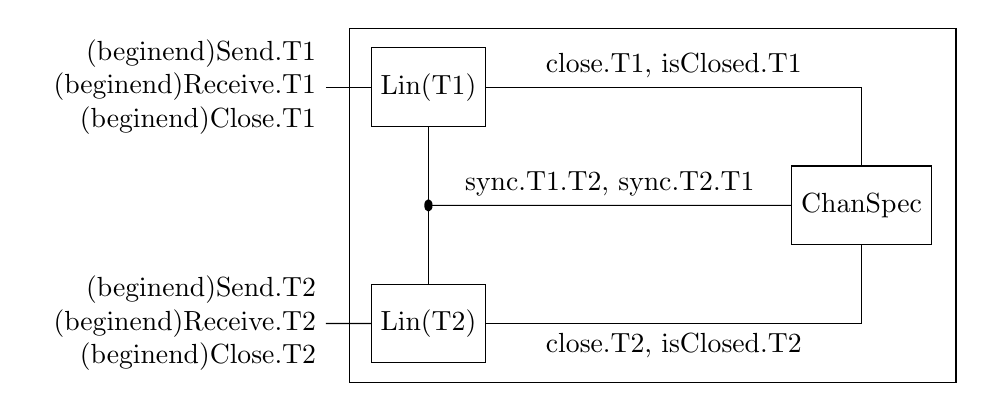
\begin{tikzpicture}[yscale = 1.5]
\draw (0,0) node[draw, minimum height = \height](lin1){\cspmstyle Lin(T1)};
\draw (0,-2) node[draw, minimum height = \height](lin2){\cspmstyle Lin(T2)};
\draw (5.5,-1) node[draw, minimum height = \height](chanSpec){
  \cspmstyle ChanSpec};
% inter-process events
\draw (lin1) -- (lin2); 
\fill (0,-1)  circle(1.5pt) coordinate (T1);
\draw (T1) -- node[above]{{\cspmstyle sync.T1.T2}, {\cspmstyle sync.T2.T1}}
   (chanSpec);
\draw (lin1) -| node[near start, above]{
  {\cspmstyle close.T1}, {\cspmstyle isClosed.T1}}  (chanSpec);
\draw (lin2) -| node[near start, below]{
  {\cspmstyle close.T2}, {\cspmstyle isClosed.T2}}  (chanSpec);
% outer box
\draw (-1,0.5) -- (6.7,0.5) -- (6.7,-2.5) -- (-1,-2.5) -- (-1,0.5);
% begin, end events
\draw (-3.2,0) node (be1) {
  \begin{tabular}{r@{}}
  \CSPM{(begin}\m\CSPM{end)Send}.\CSPM{T1} \\ 
  \CSPM{(begin}\m\CSPM{end)Receive}.\CSPM{T1} \\
  \CSPM{(begin}\m\CSPM{end)Close}.\CSPM{T1}
  \end{tabular}};
\draw(be1.east) -- (lin1);
\draw (-3.2,-2) node (be2) {
  \begin{tabular}{r@{}}
  \CSPM{(begin}\m\CSPM{end)Send}.\CSPM{T2} \\ 
  \CSPM{(begin}\m\CSPM{end)Receive}.\CSPM{T2} \\
  \CSPM{(begin}\m\CSPM{end)Close}.\CSPM{T2}
  \end{tabular}};
\draw(be2.east) -- (lin2);
\end{tikzpicture}
\end{center}
\caption{Construction of the specification process, with two threads.  We use
  BNF-style notation to capture channels with similar names; for example, we
  write ``{\cspmstyle (begin}\m{\cspmstyle end)Send}'' to denote the
  {\cspmstyle beginSend} and {\cspmstyle endSend} channels.}
\label{fig:closable-spec}
\end{figure}

We combine the linearisers as before (with suitably extended alphabets).  We
then synchronise them with |ChanSpec| on the relevant events.
events.
%
\begin{cspm}
AllLins = **|| t <- ThreadID @ [alphaLin(t)] Lin(t)
Spec£$_0$£ = AllLins [| alphaChanSpec |] ChanSpec
\end{cspm}
%
This is illustrated in Figure~\ref{fig:closable-spec} in the case of two
threads.

%
For example, |Spec|$_0$ allows traces such as
\[
\begin{align}
\trace{
  \CSPMM{C::beginSend.T1.A},\; \CSPMM{C::beginReceive.T2},\;
  \CSPMM{C::beginClose.T3},\; 
  \CSPMM{sync.T1.T2.A},\; \CSPMM{close.T3},
\\
\qquad  \CSPMM{C::endSend.T1.SendSuccess},\; 
  \CSPMM{C::endReceive.T2.ReceiveSuccess.A},\; \CSPMM{C::endClose.T3}
}.
\end{align}
\]
Here |T1| is trying to send, |T2| is trying to receive, and |T3| is trying to
close the channel; the synchronisation between~|T1| and~|T2| happens before
the |close| has an effect, so the threads successfully communicate.  But
|Spec|$_0$ also allows traces such as

\[
\begin{align}
\trace{
  \CSPMM{C::beginSend.T1.A},\; \CSPMM{C::beginReceive.T2},\;
  \CSPMM{C::beginClose.T3},\; 
  \CSPMM{close.T3},\; \CSPMM{isClosed.T1},\; \CSPMM{isClosed.T2},
\\
\qquad  \CSPMM{C::endSend.T1.Closed},\; 
  \CSPMM{C::endReceive.T2.Closed},\; \CSPMM{C::endClose.T3}
}.
\end{align}
\]
Here the channel is closed before |T1| and~|T2| can synchronise, so both
return the |Closed| value.

We can then define the specification process
\begin{cspm}
Spec = Spec£$_0$£ \ alphaChanSpec
\end{cspm}
Thus |Spec| allows all traces, containing the |begin| and |end| events, that
are synchronisation linearisable.  So testing \CSPM{Spec [T= System}
%] bracket match hack
verifies synchronisation linearisability for this system.  Performing the
corresponding test in the stable failures model also verifies synchronisation
progressibility.  Finally, performing the test in the failures-divergences
model also verifies that all assertions in the code pass, and that threads
cannot perform an infinite amount of internal activity without a thread
returning.

%%%%%%%%%%%%%%%%%%%%%%%%%%%%%%%%%%%%%%%%%%%%%%%%%%%%%%%

\subsection{Timed operations}
\label{sec:syncchan-timed}

\inlineScala

We now consider the timed send and receive operations on channels.  

The SCL conditions described earlier provide a timed wait operation: the
thread waits until either it receives a signal, or the time is elapsed; the
operation returns a boolean indicating whether a signal was received.  The
timed send and receive operations are based around this. 

The |sendWithin(duration)(x)| operation initially waits on |slotEmptied| until
either |status| holds |Empty| or the channel is closed (which it rechecks when
it receives a signal), or the deadline is reached.  If the channel is closed,
it throws a |Closed| exception.  If it timed out, it returns |false|.
Otherwise, it continues as in the untimed operation, except it waits on
|continue| until at most |duration| after the initial call.  If it then finds
that |status| is |Read|, then the send has been successful; it continues as in
the untimed operation, and returns |true|.  Otherwise |status| must still hold
|Filled| and |value| must still hold~|x| (the implementation asserts this, and
the analysis below checks this).  If the channel is closed, it continues as in
the untimed operation.  Otherwise, it must have timed out, so it sets |status|
to |Empty| to clear its value, signals to any thread waiting on |slotEmptied|,
and returns |false|.

The |receiveWithin(duration)| operation acts much as the untimed version,
except it waits on |slotFull| until at most |duration| after the initial
call.  If it then finds that |status| holds |Filled|, it continues as in the
untimed case, returning a suitable |Some| value.  If the channel is closed, it
throws a |Closed| exception.  Otherwise it must have timed out, so returns
|None|.  

%%%%% Modelling

We now describe the CSP model of these operations.  Our model and subsequent
analysis do not consider absolute time; thus we abstract away from the
duration of a timed send or receive.  The difficult part of the implementation
is getting the synchronisations right, rather than the length of the delay.

The CSP model of an SCL monitor, described in
Section~\ref{sec:basic-csp-model}, also models timed waits, via a function
|TimedAwait|.  A thread that calls this function might receive a signal, as
for untimed waits.  In addition, it can time out.  Thus we model that such
threads can eventually time out, but, as noted above, don't model the length
of the delay.


%% earlier, can be extended to also
%% model timed waits.  It records which threads are doing timed waits on which
%% conditions.  Such threads can receive a signal, as for untimed waits.  In
%% addition, they can time out, and subsequently acquire the lock on the monitor.
%% Thus we model that such threads can eventually time out, but, as noted above,
%% don't model the length of the delay.
%% , so we abstract away from the duration of a timed send or
%% receive.  The difficult part of the implementation is getting the
%% synchronisations right, rather than the length of the delay.

The |sendWithin| and |receiveWithin| operations can then be modelled in CSP
much as before, using these timed waits.


%%%%% Analysis

\inlineCSP

We adapt the specification of synchronisation linearisability as follows.  We
introduce events |timeout.t| to represent the linearisation point of a
\SCALA{sendWithin} or \SCALA{receiveWithin} operation by thread~|t| that times
out (again abstracting away from the length of the delay).  We then adapt the
definition of the lineariser processes for these operations as follows, adding
the possibility of such a time out to the possibilities of the untimed
operations.
%
\begin{cspm}
Lin(t) = 
  ... -- as before
  [] C::beginSendWithin.t?x -> SendingWithinLin(t, x, C::endSendWithin.t)
  [] C::beginReceiveWithin.t -> ReceivingWithinLin(t, C::endReceiveWithin.t)

SendingWithinLin(t, x, endChan) = 
  SendingLin(t, x, endChan)
  [] timeout.t -> endChan.Timeout -> Lin(t)

ReceivingWithinLin(t, endChan) = 
  ReceivingLin(t, endChan) 
  [] timeout.t -> endChan.Timeout -> Lin(t)
\end{cspm}
%
Further, we adapt the |ChanSpec| process to allow |timeout| events only before
the channel is closed.  The rest of the construction and checks are then as
before. 

\begin{window}[2,r,{
%
\vspace{0.5ex}
\begin{tabular}[b]{\|cccc\|}
Model & Threads & States  & Time\\
FD & 3  & 1.23M & 3.6s\\
FD & 4 & 92.5M  & 43s \\
F & 5 & 7.22B & 34min 
\end{tabular}
%\vspace{1ex}
},]
%
The table to the right gives statistics about the number of states explored
and the times taken to perform these checks, in different models, and for
different numbers of threads.  Each test used two data values (and this is the
case for all later checks reported in this paper).  All
experiments in this paper were performed on a 32-core server (two 2.1GHz
Intel(R) Xeon(R) Gold 6130 CPUs with hyperthreading enabled, with 512GB of
RAM).  The check with 5 threads in the failures-divergences model was beyond
the limits of this machine.  As is normally the case, the state space, and
hence the checking time, grows rapidly with the number of threads.   
\end{window}

%% It is worth mentioning an alternative approach, which turns out not to work
%% in this case.  For standard concurrent datatypes, linearisability is often
%% verified by identifying \emph{linearisation points}: specific points in the
%% program code where an operation execution appears to take place.  By
%% analogy, can we identify \emph{synchronisation points} in the program code
%% for each operation, where the thread is aware of the result of the
%% execution, and then capture the correctness condition in terms of these
%% synchronisation points?  More precisely, we would like identify particular
%% events in the thread processes that represent the linearisation points.

%% This idea won't work in this case, essentially because the synchronisation
%% point for one thread might depend upon what happens in other threads, whereas
%% this idea requires \emph{fixed} synchronisation points.  The synchronisation
%% point for the sending thread would have to be after it receives the signal on
%% \SCALA{continue} and regains the lock, because it doesn't know the result of
%% the synchronisation before this; but this might be too late, because the
%% channel might have been closed before it obtained the lock, and so the
%% synchronisation would appear incorrect.
